\chapter{Implementation}\label{C:impl}

\section{Front End}  %this needs a better title, badly.

web application, written using javascript, css and html5.

Figure \ref{overview} shows an overview of the Honeynet dataset. In a column to the left, we have some controls for the visualisation. To the right, taking up the majority of space is a timeline visualisation of logged data.  
<Explain basic interactions here, related back to functional and nonfunctional requirements. >
<explain why features were cut, here or design?>

Both date boxes are linked to datepicker tools, which allow for chosing a date from a calendar, and setting time through sliders. These values may be freely edited without reloading data. The Jump to dates button will trigger a reload of data. 
Binlength (Immediately below date controls) allows chosing the length of each timebin. the dropdown controls units (from seconds to years), while the textbox accepts a number of units.
<Complete detailed description>
\begin{figure}[h!]
\fbox{\parbox[b]{.99\linewidth}{
\centering 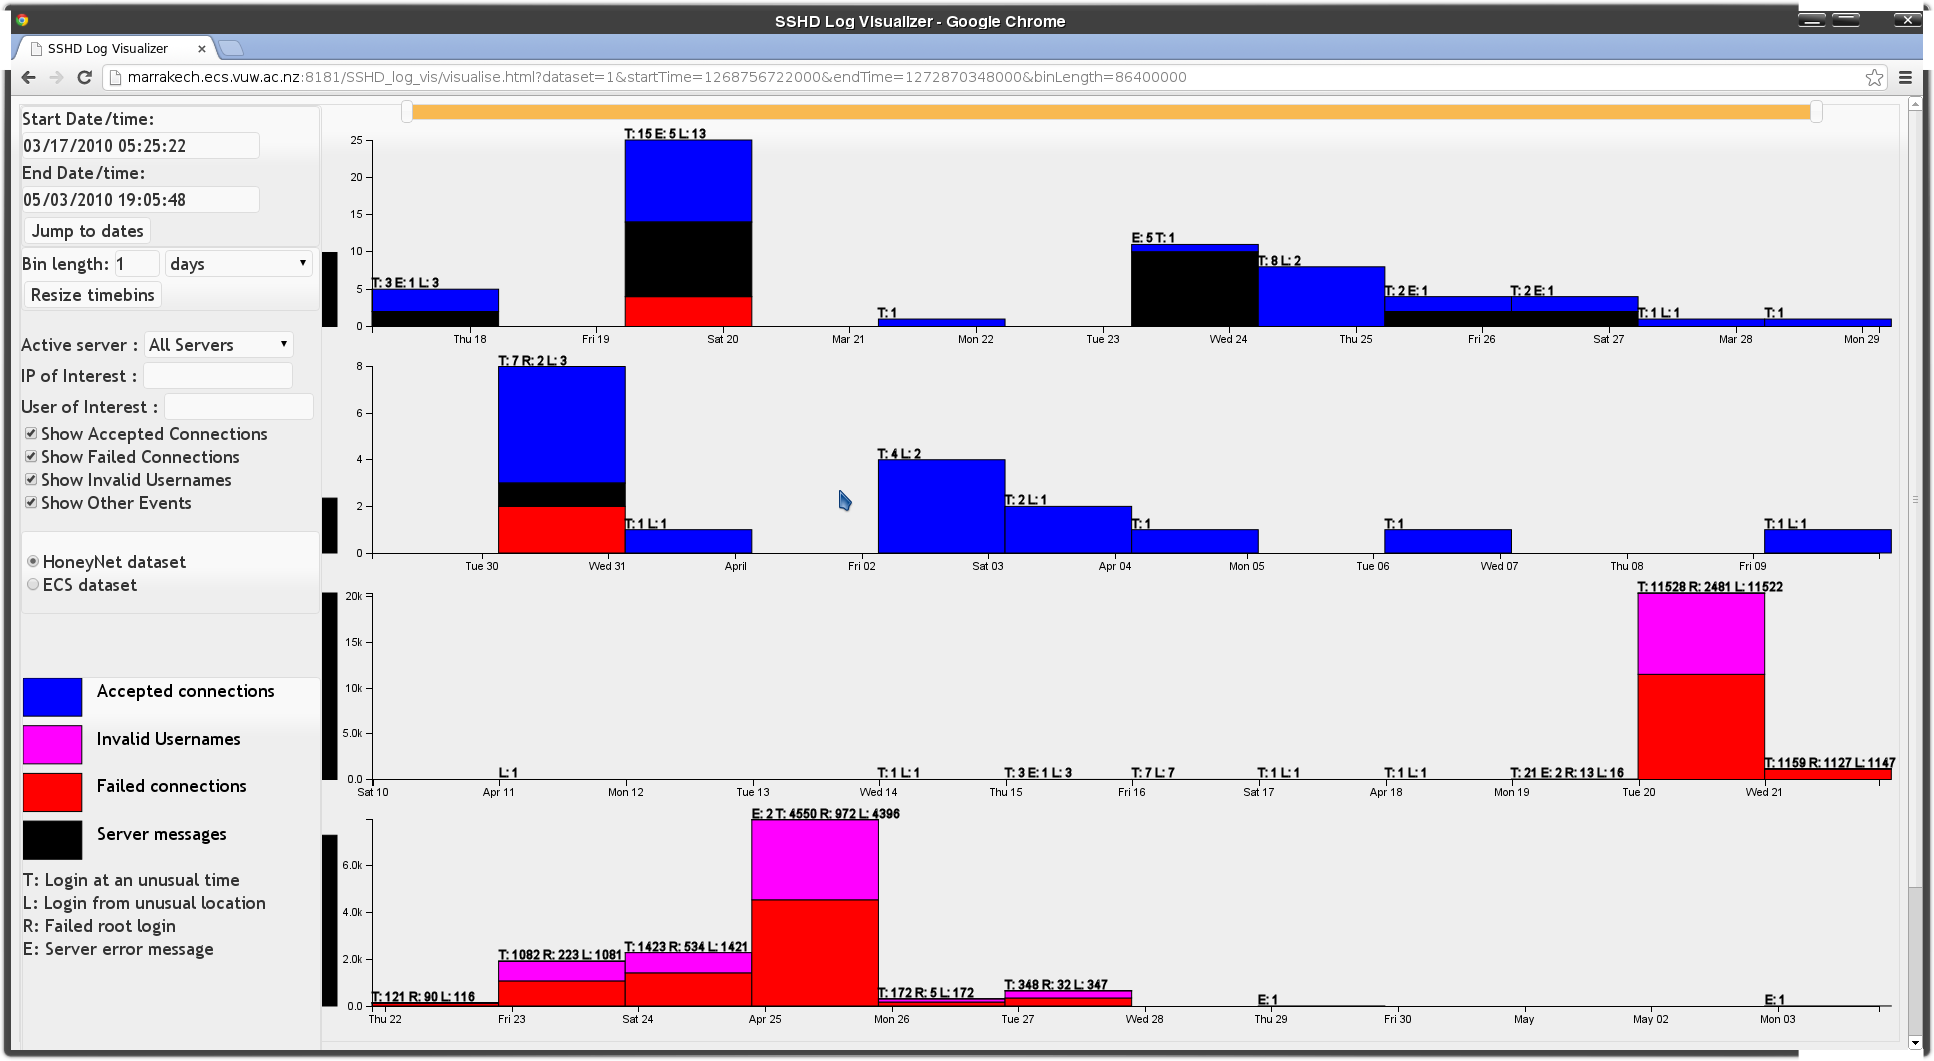
\includegraphics[scale=0.43,  angle=270]{screenshots/overview.png}
}}
\caption{\protect\label{overview}Tool showing overview of the honeynet dataset (\ref{data})}
\end{figure}


\section{Database}\label{imp_db}
Few issues were encountered with the MySql RDBMS used for the project. Two major issues arose, both causing severe performance problems for the parsing tool. One issue was related to index use for range queries, the other represented a limitation of the default java database connection system. 

GeoIp data presented a significant problem during the implementation phase of this project. I made use of the free GeoLite geoIp database, which is provided as a pair of CSV files. IP addresses in this database are represented as 32 bit unsigned integers, with a start and end column defining a range.

The extreme slowness of these queries caused unacceptable performance for the parser due to use of GeoIP information during location clustering. For batch loads potentially tens of thousands of queries would be made to the GeoIP table. Honeynet data consists of 35006 rows, of which 20469 rows resulted in GeoIp lookup. In the ECS dataset, 14885 of 75K rows resulted in GeoIp lookups. 

This design has some unfortunate implications for query efficiency, as there are approximately 2 million ranges<look up the exact number>. Range queries across two columns (constant between ColumnA and ColumnB) cannot use an index in most RDBMS systems. This results in very poor performance for queries.
Some simple optimizations are possible, assuming that ranges are non overlapping, and exhaustive. (ie: every address is in exactly 1 range)  With this assumption, a simple query selecting the first range where IP greater than or equal start, in increasing order by start will always select the matching range.

However it's uncertain if the ranges in the dataset are both exhaustive and non overlapping. Checking this property would take significant time and effort, and would need to be repeated  every time the dataset is updated (Monthly). Due to these issues, an alternative approach was sought, and found in the spatial extensions.

Using spatial extensions allows encoding the start and end numbers for IP ranges as a single shape, either line segment or square. Once so encoded, an IP can be range checked by creating a point from the address, and checking if the point is in any shapes. While this shape checking test is slower than a simple inequality test, the ability to use indexes improves performance significantly. Without spatial extensions, a range query may take many seconds, With spatial encoding this dropped to under 0.1 seconds.  

One drawback to spatial extensions for MySql is that they are not supported in the innoDB storage engine, which is the only MySql storage engine to offer transaction support. This is not a significant issue for GeoIP data, where all accesses are reads, exept for a complete table reload each time that the dataset is updated. This reload can be performed in under 5 minutes using batch loading tools available with MySql. As GeoIp databases are often updated only monthly or less frequently, this is an acceptable limitation. 

Shifting to spatially encoded ranges for GeoIp lookups was responsible for a significant improvement in loading times for batch loads. A further significant improvement was achieved by collecting groups of 1000 rows per insert transaction, as transaction overhead for the default JDBC autocommit behaviour was negatively impacting performance. 
 
\section{Parser}

The log parsing tool was implemented in two layers. A log reader, and database writer/analyser. 
The reader layer is responsible for reading any number of log files into a sorted list of events.
This list of events is then passed to the analyser/writer layer, which is responsible for checking connection attempts to see if the location and time are frequently used by the user and writing the analysed metadata to the datastore.

The writer layer is tightly coupled to both the database schema, and RDBM systems specifically as it makes extensive use of the JDBC api for communicating with RDBMS's.

Few significant issues were encountered in writing the parser. 
The majority of trouble encountered with the parser was in analysing connection attempts. checking weather a location  is one that is well known is extremely simple, though had significant performance issues discussed in \ref{imp_db}
Time clustering has proven to have ongoing issues, where overlaps in stored time ranges are not properly detected. <this goes in future work, as a known bug.> This causes a significant number of false positives for unusual times. I believe that this bug is caused by an error in my SQL queries. 
<Describe algorithm here or in design?>

\section{Server}

There were few issues with server implementation, as tomcat is well documented.
Some trouble initially setting up tomcat within university systems due to outdated instructions. 
Once this was resolved, servlet api is extremely well documented, with very good online tutorials. 
There were some issues in debugging the binning code, though these were restricted to a single servlet. 


\section{Security Concerns}
Rewrite to explain security model, including server choices that allow for defence in depth.
As I'm building the tool as a client server model, accessed through the browser
there are several security concerns to be considered in a deployment of the system.
The database will contain a significant amount of privileged information about network security
such as machine names and addresses, valid account names, and authentication methods used in the system.

This data would be extremely useful to malicious users or outside intruders. 
This leads to a need to ensure that access to this database is controlled through a robust authentication system.
Ideally the web server hosting the tool should not be accessible to the outside world at all. Within the organisation's private network access should be restricted tightly to only those users with a definite need to have access. 
Secured connections must be used for all communication between client and server to limit the opportunity for malicious individuals to snoop on the data in transit.

Security of the serverside code will be considered from the beginning of the design and implementation process
as this code must be able to resist any malicious access attempts. Through input sanitation and bounds checking should serve to close the majority of possible vulnerabilities.

Client side code contains no data, and so is significantly less critical to secure, as the database systems should deny access without valid credentials. Ideally host based authentication could be used. However, implementing a robust access control scheme does not fit within the scope of this project, and will be left for future development.


\section{Testing}
Automated testing of user interfaces remains problematic, with many tools suffering from severe fragility where UI layout is modified. In most testing libraries, mous interaction is recorded at test design, then played back artificially on execution, This causes severe fragility as if a control or button moves the recorded mouse movements will miss the button, causing test failures. Further research is needed to find a testing library suitable for testing, however the test automation tool created by Dojo appears useful \cite{dojo2013test}. - automated testing not used. heavy use of in browser dev tools and debugger. manual testing. 

\begin{figure}[tbh]
\fbox{\parbox[b]{.99\linewidth}{
\vskip 0.5cm
\centering 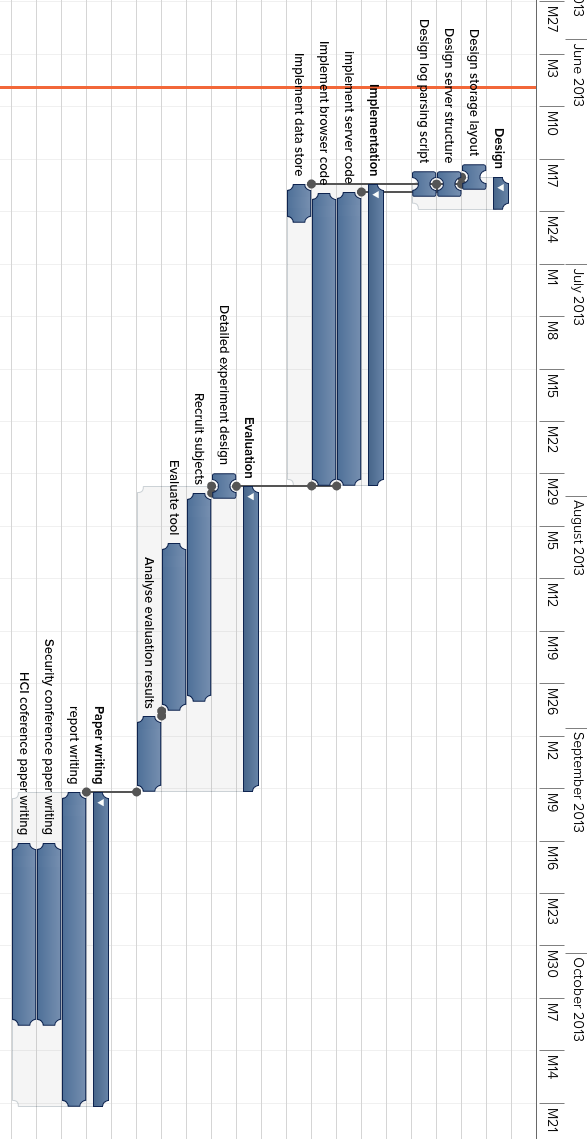
\includegraphics[scale=0.75]{gantt.png}
\vskip 0.5cm}}
\caption{\protect\label{gantt}Gantt chart showing breakdown of future work into major sections. The design group is all sub day tasks.}
\end{figure}